\documentclass[final, 10pt]{report}
\usepackage[utf8]{inputenc}
\usepackage[french]{babel}
\usepackage[top=2cm,bottom=2cm,left=2cm,right=2cm]{geometry}
\usepackage[style=numeric,backend=biber]{biblatex}
\usepackage{hyperref}
\usepackage{graphicx}
\usepackage[T1]{fontenc}
\usepackage{amssymb}
\usepackage{amsmath}
\usepackage{algpseudocode}
\usepackage{algorithm}
\usepackage{subcaption}

\setlength{\parskip}{5pt}

\addbibresource{Recherche_Documentaire_2022.bib}

\title{Recherche documentaire}
\author{\textsc{Cuenin} Tommy\and \textsc{Grosdidier} Alphée}
\date{Juin 2022}


\makeatletter
\def\maketitle{
  \newpage
  \null
  \vskip 2em
  {\raggedright 
\includegraphics[scale=0.2]{img/nom_universite.png}\hspace{\stretch{1}}
\includegraphics[scale=0.4]{img/reseauFigure.png}}
  \begin{center}
  \let \footnote \thanks
    {\Huge \textbf{\@title} \par}
    \vskip 1.5em%
    {\Large%
    \textbf{Complétion (semi-)automatique}
    }%
    \vskip 1.5em%
    {\large
      \lineskip .5em%
      \begin{tabular}[t]{c}
        \@author
      \end{tabular}\par}
      \vskip 3em%
    {\Large Enseignant encadrant: Pierre-Cyrille \textsc{Héam}}%
    \vskip 1em%
    \vspace{\stretch{1}}
    {\large%
    Cursus Master en Ingénierie}
    \vskip 1.5em
    {\large Année 2021~-2022}%
  \end{center}%
  \par
  \vskip 1.5em
  \pagestyle{empty}}
\makeatother

\begin{document}

\maketitle

\tableofcontents

\chapter{Étude de différentes approches utilisées.}
\section{Introduction}
    %Ceci est un premier jet : il faut le retravailler
    Selon l'article de \emph{Wikipedia} \cite{noauthor_auto-completion_2019} \og\emph{L'auto-complétion ou autocomplétion ou complétion automatique, souvent simplement complétion, parfois complètement ou complètement automatique, est une fonctionnalité informatique permettant à l'utilisateur de limiter la quantité d'informations qu'il saisit avec son clavier, en se voyant proposer un complément qui pourrait convenir à la chaîne de caractères qu'il a commencé à taper.}\fg{}
    
    La complétion (semi-)automatique a pour but de nous simplifier la tâche d'écriture en corrigeant nos erreurs, en proposant différents mots suivant les premières lettres saisies ainsi qu'en nous proposant d'écrire des mots complets en \textit{un} clic.
    Elle permet une augmentation de la vitesse de saisie d'un texte et assure un respect des règles linguistiques de la langue choisie.
    
    Cette technologie est intégrée à toutes nos tâches d'écriture quotidiennes comme les rapports, mails, messages, ou encore l'écriture de code etc. Grâce à l'optimisation constante des programmes et à une meilleure compréhension du langage par les ordinateurs on est en mesure d'implémenter ces outils sur des appareils très peu puissants comme les téléphones portables tout en ayant une bonne efficacité.
    
    Présente sur la plupart des téléphones, elle augmente significativement la vitesse de saisie de texte en corrigeant les fautes de frappe et d'orthographe et en recommandant des termes, ce qui permet l'économie de la saisie de mots parfois longs. Ce gain de temps est d'autant plus significatif dans des langues où l'on peut écrire un mot composé en un seul bloc comme en allemand (par exemple :  die Messe + die Halle = die Messehalle  =  le hall d'exposition).

\footnotesize
sources : 
\begin{itemize}
    \item \url{https://en.wikipedia.org/w/index.php?title=Predictive_text&oldid=1056470462}
    \item \url{https://fr.wikipedia.org/w/index.php?title=Auto-compl\%C3\%A9tion&oldid=165592185}
    \item \url{https://en.wikipedia.org/w/index.php?title=Autocomplete&oldid=1062628465}
\end{itemize}
\normalsize

\section{Histoire}

    L’histoire des correcteurs automatiques a commencé chez \emph{Microsoft} au début des années 90, avec \emph{Dean Hachamovitch}.
    A cette époque le logiciel Word n'avais qu'un \og autoexpander\fg{}, des raccourcis clavier pour écrire un mot pré-enregistré.
    Alors \emph{Dean Hachamovitch} s'est inspiré de ce système pour créer le premier mécanisme de correction connue.
    Ce logiciel remplaçait tous les \og teh\fg{} par \og the \fg{}.
    
    \emph{Hachamovitch} et son équipe ont vu que c'était une idée intéressante.
    Les années suivantes ils ont recensé les erreurs orthographiques et typographiques les plus courantes.
    Cependant le logiciel ne pouvait corriger que les fautes déjà été signalées et corrigées par l'équipe de \emph{Microsoft}.
    
    
    Le bouillonnement technologique de la fin des années 90 a vite apporté un début de solution au problème de Hachamovitch. Le fameux T9 ou « Texte sur neuf touches » de Cliff Kushler, le co-fondateur de l’entreprise Tegic Communications, mêlait le système de dictionnaire des logiciels de traitement de texte à des formules d’apprentissage des habitudes rédactionnelles des utilisateurs des premiers téléphones portables. La saisie intuitive était née. Taper des messages sur un clavier à neuf touches devenait soudain plus facile et rapide.En 1999, la popularité des SMS explosait, un Américain envoyait en moyenne 0,4 messages par mois\ldots Et 35 cinq ans plus tard.
    \cite{wesolowski_les_2021}

\footnotesize
sources : 
\begin{itemize}
    \item \url{https://en.wikipedia.org/w/index.php?title=Predictive_text&oldid=1056470462}
    \item \url{https://fr.wikipedia.org/w/index.php?title=Auto-compl\%C3\%A9tion&oldid=165592185}
    \item \url{https://www.vice.com/fr/article/7k93be/les-correcteurs-automatiques-ne-seront-jamais-bons}
\end{itemize}
\normalsize

\section{Par dictionnaire}

    La (semi-)complétion automatique par dictionnaire est la première approche à avoir été utilisée sur téléphone.
    A l'époque du \og T9\fg{} les applications pouvant tourner sur téléphones étaient très limitées en puissance de calcul et devaient donc être peut gourmandes en ressources tout en restant rapides. 
    L'approche par dictionnaire est assez simple puisqu'il suffit d'un dictionnaire composé de tous les mots de la langue correctement orthographiés et d'un bon algorithme de distance d'édition.
    
    
    Avec cette approche on vérifie si le mot est contenu dans le dictionnaire sinon on cherche le mot possible le plus proche avec le moins de caractères différents. 
    Dans l'exemple du T9 on met en priorité les changements avec les lettres qui sont sur les même touches. 
    Avec un clavier ce serait avec les touches qui se trouvent autour de la touche appuyée.
    
    
    On utilise aussi un dictionnaire utilisateur afin de pouvoir ajouter à la liste des mots préenregistrés les mots de l'utilisateur qui ne s'y trouvent pas.
    
    Le problème lié à cette approche est que le dictionnaire de la langue doit être maintenu à jour très régulièrement. Ce qui rend difficile la maintenance du programme. De plus il est compliqué de répertorier tous les mots notamment le \og verlent \fg{} ou les mot raccourcis dans les \og textos \fg{}.
    
    Cette approche ne permet pas non plus de prendre en compte le contexte de la phrase ou du texte en général ce qui rend cette approche limitée. On peux l'utiliser pour corriger des mots mais une relecture humaine est souvent nécessaire voire obligatoire.

    sources : 
    \begin{itemize}
        \item \url{https://en.wikipedia.org/w/index.php?title=Predictive_text&oldid=1056470462}
    \end{itemize}

\section{Par mot précédemment saisis}

    Les suggestions données à l'utilisateur peuvent se baser sur son propre vocabulaire. En effet on peut supposer que l'utilisateur sera amené à réutiliser des mots qu'il a déjà utilisé, la question sera donc de déterminer quels sont les mots qu'il réutilisera à l'avenir.
    En moyenne une personne française utilise 300 à 5 000 mots\cite{admin6658_combien_2020} sur 32 000 mots couramment utilisés\cite{noauthor_combien_nodate} dans la langue française sur un total de 90 000 mots.
    On peux ainsi avoir des propositions de mots beaucoup plus rapides et justes en se basant simplement sur les 5 000 mots que la personne utilise.
    On peut lier une correction avec un dictionnaire des mots pour avoir une base de mots correctement écrits (puisqu'on veut corriger les textes) et proposer ensuite les mots que l'utilisateur veux écrire avec son historique.
    
    Cependant cette approche pose le problème de savoir comment ces données vont être utilisées puisqu'elles sont enregistrées sur son téléphone mais pourraient très bien être récupérées par le créateur du logiciel.
    Ces données peuvent ensuite améliorer le logiciel ou être utilisées à des fins commerciales.
    
    \footnotesize
    sources :
    \begin{itemize}
        \item \url{https://www.intercountry.com/blog/combien-de-mots-dans-la-langue-francaise}
        \item \url{https://plumelibre.fr/2020/08/combien-de-mots-utilise-t-on/}
    \end{itemize}
    \normalsize

\section{Par les caractères de l'application}

    Certains termes ne sont utilisés que dans certains cas comme par exemple une adresse mail.
    Certains ne se trouvent pas dans le dictionnaire et donc un logiciel de complétion (semi-)automatique aura des difficultés à les corriger.
    On a donc décidé d'utiliser les informations des applications pour compléter le dictionnaire de mots.
    Comme l'exemple cité précédemment l'application de mails va récupérer les mails enregistrés pour corriger les adresses mails saisies.
    
    Sur les téléphones on utilise aussi cette approche pour les noms des contacts, en effet, les noms propres ne figurant pas dans le dictionnaire, ils seraient interprétés comme des erreurs et corrigés en vain. Cela permet à la fois d'éviter leur correction inutile ainsi que de corriger en cas d'erreur d'écriture du nom.
    
    \footnotesize
    source : \url{https://www.twaino.com/definition/a/autocompletion/}
    \normalsize
    
\section{Par sémantique}

    Avec l'amélioration de la puissance et de la mémoire du matériel, une approche sur l'ensemble d'une phrase, voire d'un texte, a pu voir le jour.
    On décrira successivement les approches qui sont apparues pour pouvoir faire une prédiction de texte de plus en plus pertinente.
    
    \subsection{Intelligence artificielle}
    
        Une nouvelle approche qui a fait surface depuis quelques années est celle de l'intelligence artificielle.
        Le principe est de travailler avec un réseau neuronal (On ne prendra pas le temps d'expliquer en détails leurs fonctionnement).
        On met en entrée les mots de la phrase et le réseau neuronal entraîné nous sort les meilleurs mots pour compléter celle-ci. % le réseau neuronal propose les mots les plus adaptés
        
        Mais on se retrouve face à plusieurs problèmes. 
        Dans un premier temps, si on prend en entrée les mots on a des dizaines de milliers d'entrées et de sorties ce qui est assez lourd pour le traitement.
        Puis pour les noms, qui sont spécifiques à chaque utilisateur, ils n'ont pas forcément leur entrée ni leur sorties dans dans ce type d'intelligence artificielle.
        
        On serait donc tenté de prendre chaque lettre en entrée et sortie mais le problème qui apparaît est que le risque d'avoir des mots qui n'existent pas dans la langue.
        On a donc réfléchi à une autre approche en gardant l'intelligence artificielle qui promet de meilleurs résultats que l'approche statique.
        
        \footnotesize
        source : \url{http://arxiv.org/abs/2201.06892}
        \normalsize
    
    \subsection{Algorithme GPT-3}

        L'algorithme GPT est développé par \textbf{OpenIA}, l’entreprise de recherche en IA co-fondée par Elon Musk\cite{noauthor_quest_2021}.
        Elle est basée sur une réelle analyse sémantique cherchant à reconnaître la valeur des mots.
        
        Par exemple dans la phrase: \og J'ai acheté du chocolat à Auchan pour le gâteau d'anniversaire de Jane \fg{}, l'algorithme reconnaîtra le mot \og Auchan \fg{} comme nom de marque et \og Jane \fg{} comme celui d'une personne.
        Cette analyse permet ensuite à un réseau neuronal de prédire la suite de la phrase de façon pertinente.
        Nous ne rentrons pas plus dans les détails mais il est important de noter que pour entraîner cet intelligence artificielle, cette organisation aurait dépensé près de 4,6 millions de dollars\cite{noauthor_quest_2021} et prendrait en compte 175 milliards de paramètres\cite{noauthor_quest_2021}.
        On est donc pas près de voir tourner cet algorithme sur nos téléphones portables autrement qu'à l'aide d'une connexion avec une machine assez puissante.

\chapter{Étude des algorithmes de calcul de distance, par exemple de distance d’édition.}


\begin{figure}
    \centering
    \begin{subfigure}{0.4\textwidth}
        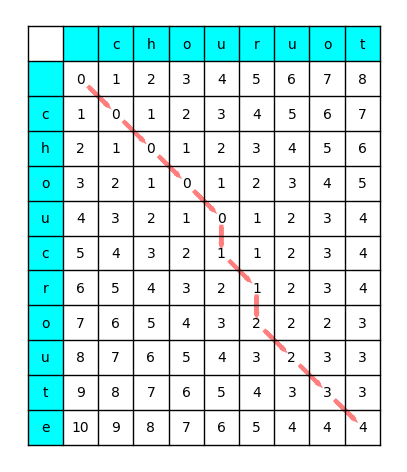
\includegraphics[width=.90\textwidth]{img/Tableau_de_Levenshtein.png}
        \caption{Tableau de Levenshtein}
        \label{fig:tab_levensthein}
    \end{subfigure}
    \begin{subfigure}{0.4\textwidth}
        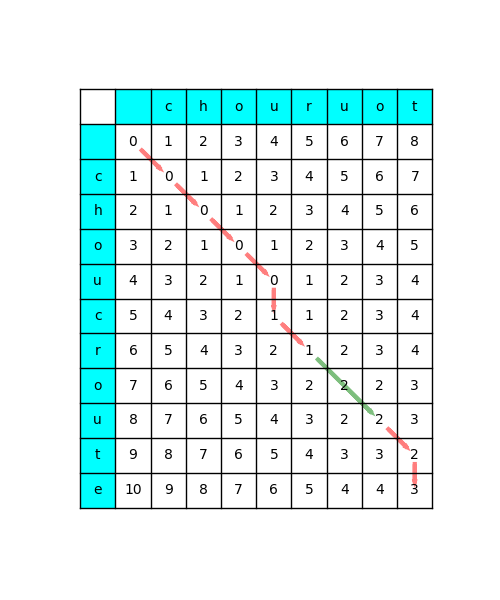
\includegraphics[width=.90\textwidth]{img/Tableau_de_Damerau-Levenshtein.png}
        \caption{Tableau de Damerau-Levenshtein}
        \label{fig:tab_damerau}
    \end{subfigure}
    \caption{Algorithme type Levenshtein}
    \label{fig:algo_levensthein}
\end{figure}
    

\section{Algorithme de Levenshtein}

    L'algorithme de Levenshtein permet de calculer la distance entre deux chaînes.
    Elle quantifie la différence des deux chaînes de caractères et s'écrit sous forme mathématique $\text{lev}(C1,C2)$
    Pour ce faire, elle dispose de trois opérations fondamentales qui sont~:
    \begin{itemize}
        \item l'ajout;
        \item la suppression;
        \item la substitution de caractères.
    \end{itemize}
    
    \medskip
    Cet algorithme est considérée comme une généralisation de la distance de Hamming\cite{noauthor_distance_2021-1} qui était utilisée pour connaître le nombre de bits altérés lors de la transmission de messages dans les télécommunications.
    
    L'agorithme de Levenshtein se définit par la formule suivante~:
    
    $$
    {\displaystyle \qquad \operatorname {lev} (a,b)={\begin{cases}\max(|a|,|b|)&{\text{ si }}\min(|a|,|b|)=0,\\\operatorname {lev} (a-1,b-1)&{\text{ si }}a[0]=b[0],\\1+\min {\begin{cases}\operatorname {lev} (a-1,b)\\\operatorname {lev} (a,b-1)\\\operatorname {lev} (a-1,b-1)\end{cases}}&{\text{ sinon.}}\end{cases}}}
     $$



Par exemple pour passer de "foyer" à "loyers", il faut effectuer deux opérations :
\begin{itemize}
    \item substitution du caractère 'f' par le caractère 'l'
    \item ajout du caractère 's'
\end{itemize}
La distance de Levenshtein dans ce cas est donc de 2.

À noter que chaque opération que l'on a cité à le même poids, qui est de 1 et qu'en toute logique dans le cas où les mots sont les mêmes la distance sera 0.

L'algorithme de Levenshtein est la formalisation en langage algorithmique du calcul de distance de Levenshtein,  à l'aide d'une matrice de taille $n$+$1\times m$+$1$ avec $n$ et $m$ la taille des deux mots dont on cherche la distance.
% manque quelquechose
Voici ci-dessous un exemple d'utilisation de l'algorithme de Levenshtein pour calculer la distance entre "chouruot" et "choucroute".\ref{fig:algo_levensthein}
Le tableau fait l'inventaire de l'ensemble des chemins possibles, et à la fin subsiste le chemin minimal.
Ce dernier est donc :
\begin{itemize}
    \item suppression de 'c'
    \item suppression de 'o'
    \item substitution de 't' par 'o'
    \item substitution de 'e' par 't'
\end{itemize}
%manque quelquechose

\footnotesize source : \url{https://fr.wikipedia.org/wiki/Distance_de_Levenshtein}
\normalsize

\section{Algorithme de Damerau-Levenshtein\cite{noauthor_distance_2020}}

    L'algorithme de Damereau-Levenshtein utilise le même principe que l'algorithme de Levenshtein.
    On garde les 3 opérations de base mais on ajoute une opération supplémentaire~: la transposition.
    La transposition est l'échange de position de deux lettres côte à côte qui a le même coût qu'une opération fondamentale.
    Ainsi le mot \fg chat \og{} et \fg hcat\fg{} ont un distance d'édition de 1 au lieu de 2 avec l'algorithme de Levensthein.
    
    Ces opérations forment environ 80\% des fautes d'orthographes humaines.
    On a donc un algorithme de correction orthographique qui est assez efficace mais on est encore loin d'avoir la perfection.
    
    Si l'on reprend l'exemple précédent, la suppression de 'o' et substitution de 't' par 'o' sont remplacés par une transposition de 'r' et 'o', transformant deux opérations en une seule, ce qui réduit donc la distance à 3.
    
\begin{figure}
    \centering
    \begin{subfigure}{0.4\textwidth}
        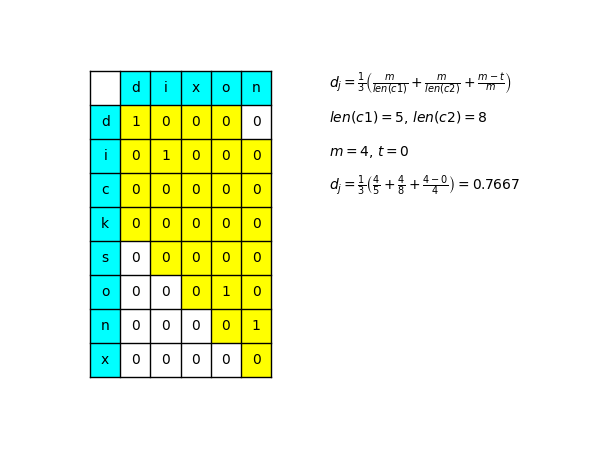
\includegraphics[width=.90\textwidth]{img/Table_de_Jaro.png}
        \caption{Tableau de Jaro}
        \label{fig:tab_jaro}
    \end{subfigure}
    \begin{subfigure}{0.4\textwidth}
        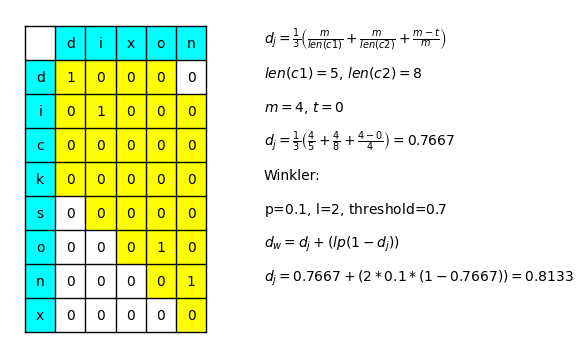
\includegraphics[width=.90\textwidth]{img/Table_de_Jaro-Winkler.png}
        \caption{Tableau de Jaro-Winkler}
        \label{fig:tab_winkler}
    \end{subfigure}
    \caption{Algorithme type Levenshtein}
    \label{fig:algo_jaro}
\end{figure}
    
\section{Algorithme de Jaro\cite{noauthor_distance_2021}}
    
    La distance de Jaro calcule le nombre de lettres qui sont présentes dans les deux mots et le nombre de lettres qui ne sont pas à la bonne place par rapport aux autres.
    
    On calcule la distance de Jaro à l'aide du calcul suivant~: 
    $$d_j = \frac{1}{3}\left(\frac{m}{\text{len}(c1)}+\frac{m}{\text{len}(c1)}+\frac{m-t}{m}\right)$$
    Où~:
    \begin{itemize}
        \item $\text{len}(ci)$ est la longueur de la chaîne $i$;
        \item $m$ est le nombre de caractères correspondants;
        \item $t$ est le nombre de transpositions
    \end{itemize}

    \medskip
    On considère que deux caractères correspondent si le caractère est présent dans les deux chaînes et que la distance les séparant est inférieure ou égale à $$\lfloor\frac{\text{max}(\text{len}(c1), \text{len}(c2)}{2}\rfloor -1$$
    
    À noter que à l'inverse de l'algorithme de Levensthein, un nombre correspondant à la distance plus élevé signifie plus de correspondances donc moins de distance.
    
    Dans l'exemple de la distance entre \og dixon\fg{} et \og dicksonx\fg{} : les caractères 'd','i','o','n' et 'x' sont communs aux deux chaînes or $$\lfloor\frac{\text{max}(\text{len}("dixon"), \text{len}("dicksonx")}{2}\rfloor -1 = \lfloor\frac{\text{max}(5,8)}{2}\rfloor -1 = 3$$
    or l'écart entre les deux 'x' est de $5 > 3$ donc on ne prend pas 'x', en compte, donc $m = 4$. On n'a aucune transposition donc $t = 0$. On calcule $$d_j = \frac{1}{3}\left(\frac{4}{5}+\frac{4}{8}+\frac{4-0}{4}\right) = \frac{23}{30} \approx 0.7667$$
    
\section{Algorithme de Jaro-Winker\cite{noauthor_distance_2021}}

    Une amélioration de l'algorithme de Jaro a été faite par William E. Winkler.
    Il a décidé de mettre plus d'importance sur la similitude des débuts de mots.
    
    On peux prendre le même exemple que précédemment avec de \og annulaire\fg{} avec \og annuaire\fg{}. 
    La distance de Jaro entre les deux mots est de $0.8630$
    Maintenant si je compare  \fg annuaire\og{} avec \fg annnuaire\og{}.
    On a une distance de Jaro de $0.8630$.
    On a ajouté simplement une lettre dans les deux chaînes.
    
    Les mots écrits humainement sont généralement bien écrits dans les premières lettres puis les fautes d'orthographes apparaissent.
    Donc pour être plus précis, William E. Winkler a décidé d'avantager les mots qui ont le plus long préfixe commun.
    
    On a donc le calcul suivant~:
    $$ d_w = d_j +(l * p * (1-d_j) )$$
    Où~:
    \begin{itemize}
        \item $d_j$ est la valeur de l'algorithme de Jaro;
        \item $l$ est la longueur du préfixe commun (maximum 4 caractères);
        \item $p$ est un coefficient qui permet de favoriser les chaînes avec un préfixe commun.
        Winkler propose pour valeur $p=0.1$
    \end{itemize}
    
    Ainsi la distance Jaro-Winker entre \fg annuaire\og{} et \fg annulaire\og{} est de $0.9778$ alors que la distance entre \fg annuaire\og{} et \fg annnuaire\og{} est de $0.9741$
    
    Cet algorithme est plutôt utilisé dans la détection de doublons mais peut aussi être une approche dans la correction automatique.\\
    
    Si l'on reprend la distance entre \og dixon\fg{} et \og dicksonx\fg{}, vu que ces deux mots on en commun \og di\fg{}, $l = 2$.
    On prend $p = 0.1$,la distance de Jaro-Winker est donc $\frac{23}{30} + \left( 2 \times 0.1 \times \left( 1 - \frac{23}{30} \right)\right) = \frac{61}{75} \approx 0.8133$.
    
\chapter{Étude (simple) de chaînes de Markov pour l’historique.}
%à revoir légèrement
Une chaîne de Markov est un processus stochastique possédant la propriété de Markov, la propriété de Markov étant que, soit un système constitué de plusieurs états, fixé sur un état à la fois et pouvant transiter vers d'autres états, la prédiction de l'état futur du système à l'instant $n$ dépend uniquement de l'état du système à l'instant présent $n-1$ et donc est indépendante des états passés à l'instant $n-k$ avec $1<k\leq n$, donc le système n'a pas de mémoire.
Ainsi la probabilité de transition d'un état à l'autre dépend uniquement de l'état duquel on provient, on écrit donc la probabilité de transition $\mathbb{P}(X_{n+1}=a | X_{n}=b)$ avec $a$ et $b$ deux états pouvant être égaux.e l
\begin{figure}[!h]
    \centering
    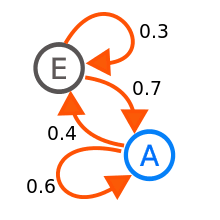
\includegraphics[scale=0.5]{img/markovChaine.png}
    \caption{Représentation d'une chaîne de Markov}
    \label{fig:chaine_markov}
\end{figure}

Les chaînes de Markov sont modélisées en mathématique par des matrices de transition qui sont des matrices carrées qui associent à chaque ligne un état initial et à chaque colonne la probabilité de transition vers un état, ainsi soit $(a,b)$ un couple d'entiers et $M$ une matrice de transition, $M_{a,b}$ est la probabilité de transition de l'état numéro $a$ à l'état numéro $b$.

La matrice de transition de la chaîne de Markov ci-dessus est la suivante (les lignes et les colonnes correspondent dans l'ordre aux états représentés sur le graphe E, A) : 

$\begin{pmatrix}
0.3 & 0.7 \\
0.4 & 0.6
\end{pmatrix}$

La somme des probabilités de chaque ligne doit être égale à 1 ce qui implique que tous les états doivent êtres connus ainsi que leur probabilité de transition.

Les chaînes de Markov sont utilisées dans beaucoup de domaines, par exemple, les chaînes de Markov sont utilisées par Google pour déterminer l'indice de popularité d'une page web à partir d'un état quelconque de la chaîne de Markov représentant le Web.

Dans le cas du sujet vu qu'un texte est une suite de mots, on pourrait partir du principe qu'un mot est un état.
Si on se sert de chaque saisie d'utilisateur pour compléter des chaînes de Markov associées, on pourrait déterminer, en se basant sur la fréquence,  quels sont les mots les plus fréquemment utilisés à la suite d'un autre et ainsi faire des propositions intéressantes.
\begin{figure}[h]
    \centering
    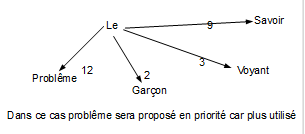
\includegraphics[scale=1]{img/Mark.png}
    \caption{Les chaines de Markov avec les mots}
    \label{fig:chaine_markov_word}
\end{figure}

% IMPORTANT prler des chaines de markov de n-ordres
Il est aussi possible de tenir compte d'un nombre $n-(k-1)$ d'états précédents fixé en plus de $n$, c'est ce qui s'appelle les chaînes de Markov de $k$-ordre, $0<k<n$. Ainsi pour l'ordre k=3, l'écriture de la probabilité de transition devient $\mathbb{P}(X_{n+1}=a | X_{n}=b , X_{n-1}=c , X_{n-2}=d)$.
En tenant compte d'un nombre défini d'états précédents on va pouvoir affiner la précision des prédictions, cependant en contrepartie la quantité d'information à fournir pour que ce soit fonctionnel et efficace est significativement plus élevée.

Par exemple, pour la prédiction d'un mot dans une phrase, alors qu'une prédiction d'ordre 1 s'appuierait sur un mot, une prédiction d'ordre 3 s'appuierait sur trois mot, ce qui implique une connaissance des probabilités qu'un mot soit à la suite d'un groupe de mot donc, pour être au mieux exhaustif, beaucoup de données.

Cependant cette approche a des limites comme l'absence de mémoire qui empêche d'affiner la recommandation de mots car cette dernière se base sur uniquement un seul mot et non l'ensemble de la phrase qui précède.

\footnotesize
source : 
\begin{itemize}
    \item \url{https://fr.wikipedia.org/wiki/Cha\%C3\%AEne_de_Markov}
    \item \url{https://yurichev.com/blog/markov/}
    \item \url{https://datascience.eu/fr/mathematiques-et-statistiques/chaines-de-markov/}
\end{itemize}
\normalsize

\printbibliography[heading=bibintoc,title={Bibliographie}]

\end{document}